\section{Background}

The ageing global population increases the need for investment in geriatrics. One area of particular significance within this field is that of rhinology. A range of dysfunctions and aberrations from the normal functioning of nasal cavities in healthy adults have been observed in the elderly population \cite{Edelstein1996, Lindemann2008}. For example, the occurrence of respiratory diseases in the elderly is markedly higher than that found in younger populations \cite{HO2001, Edelstein1996}. It has been suggested that these higher recorded rates could be due in part to the impaired air conditioning functionality \cite{Lindemann2008}.


The nasal cavities of elderly citizens exhibit increased volume \cite{Kalmovich2005}. Alterations in histiological function have also been shown \cite{HO2001}. The extent to which functional aberrations are caused by geometric (as opposed to histiological) variations remains unclear \cite{Varga-Huettner2013}. These changes in nasal physiology - and their impact on nasal functionality - need to be investigated further.


Computational Fluid Dynamics (CFD) numerically approximates flow field characteristics for a given domain. CFD simulations give highly detailed results with information covering a range of areas for a given fluid system at a minimal cost. One area in which CFD simulations have been gaining credence is that of biomechanics; many biological fluid systems can be modelled effectively through CFD simulations, allowing for an unprecedented insight into their function.

The use of 3D medical imaging techniques such as computed tomography (CT) scans in collaboration with CFD has facilitated the numerical approximation of fluid mechanism parameters in anatomically accurate models. This allows for more detailed analysis of the effects of topological variations on fluid mechanisms. This capacity for detailed comparison makes CFD simulation an ideal tool for analysing the impact of physiological discrepencies on nasal patency.


To date numerous inter-demographic studies have been carried out using CFD analysis of 3D models reconstructed from CT scan data \cite{Xi2012, Garcia2007, Zhu2011}. These studies have indicated that factors such as ethnicity and gender are liable to impact on nasal physiology. Previous studies have focused on age \cite{Xi2012}, however to date these age related studies have all focused on children. The use of CFD to examine functional variations in older models - accounting for potential interdemographic variations such as gender or ethnicity - is thus an important step that needs to be taken in order to achieve a more comprehensive understanding of the impact of ageing on nasal patency. For the sake of this thesis, the term older will be taken to mean ages of 60 and older.

\section{Literature review}
In this section the relevant literature regarding older nasal cavities will be reviewed. Significant gaps in the current body of knowledge will be identified and serve as the foundation for this thesis.

\subsection{Nasal cavity anatomy}


\begin{figure}
\centering
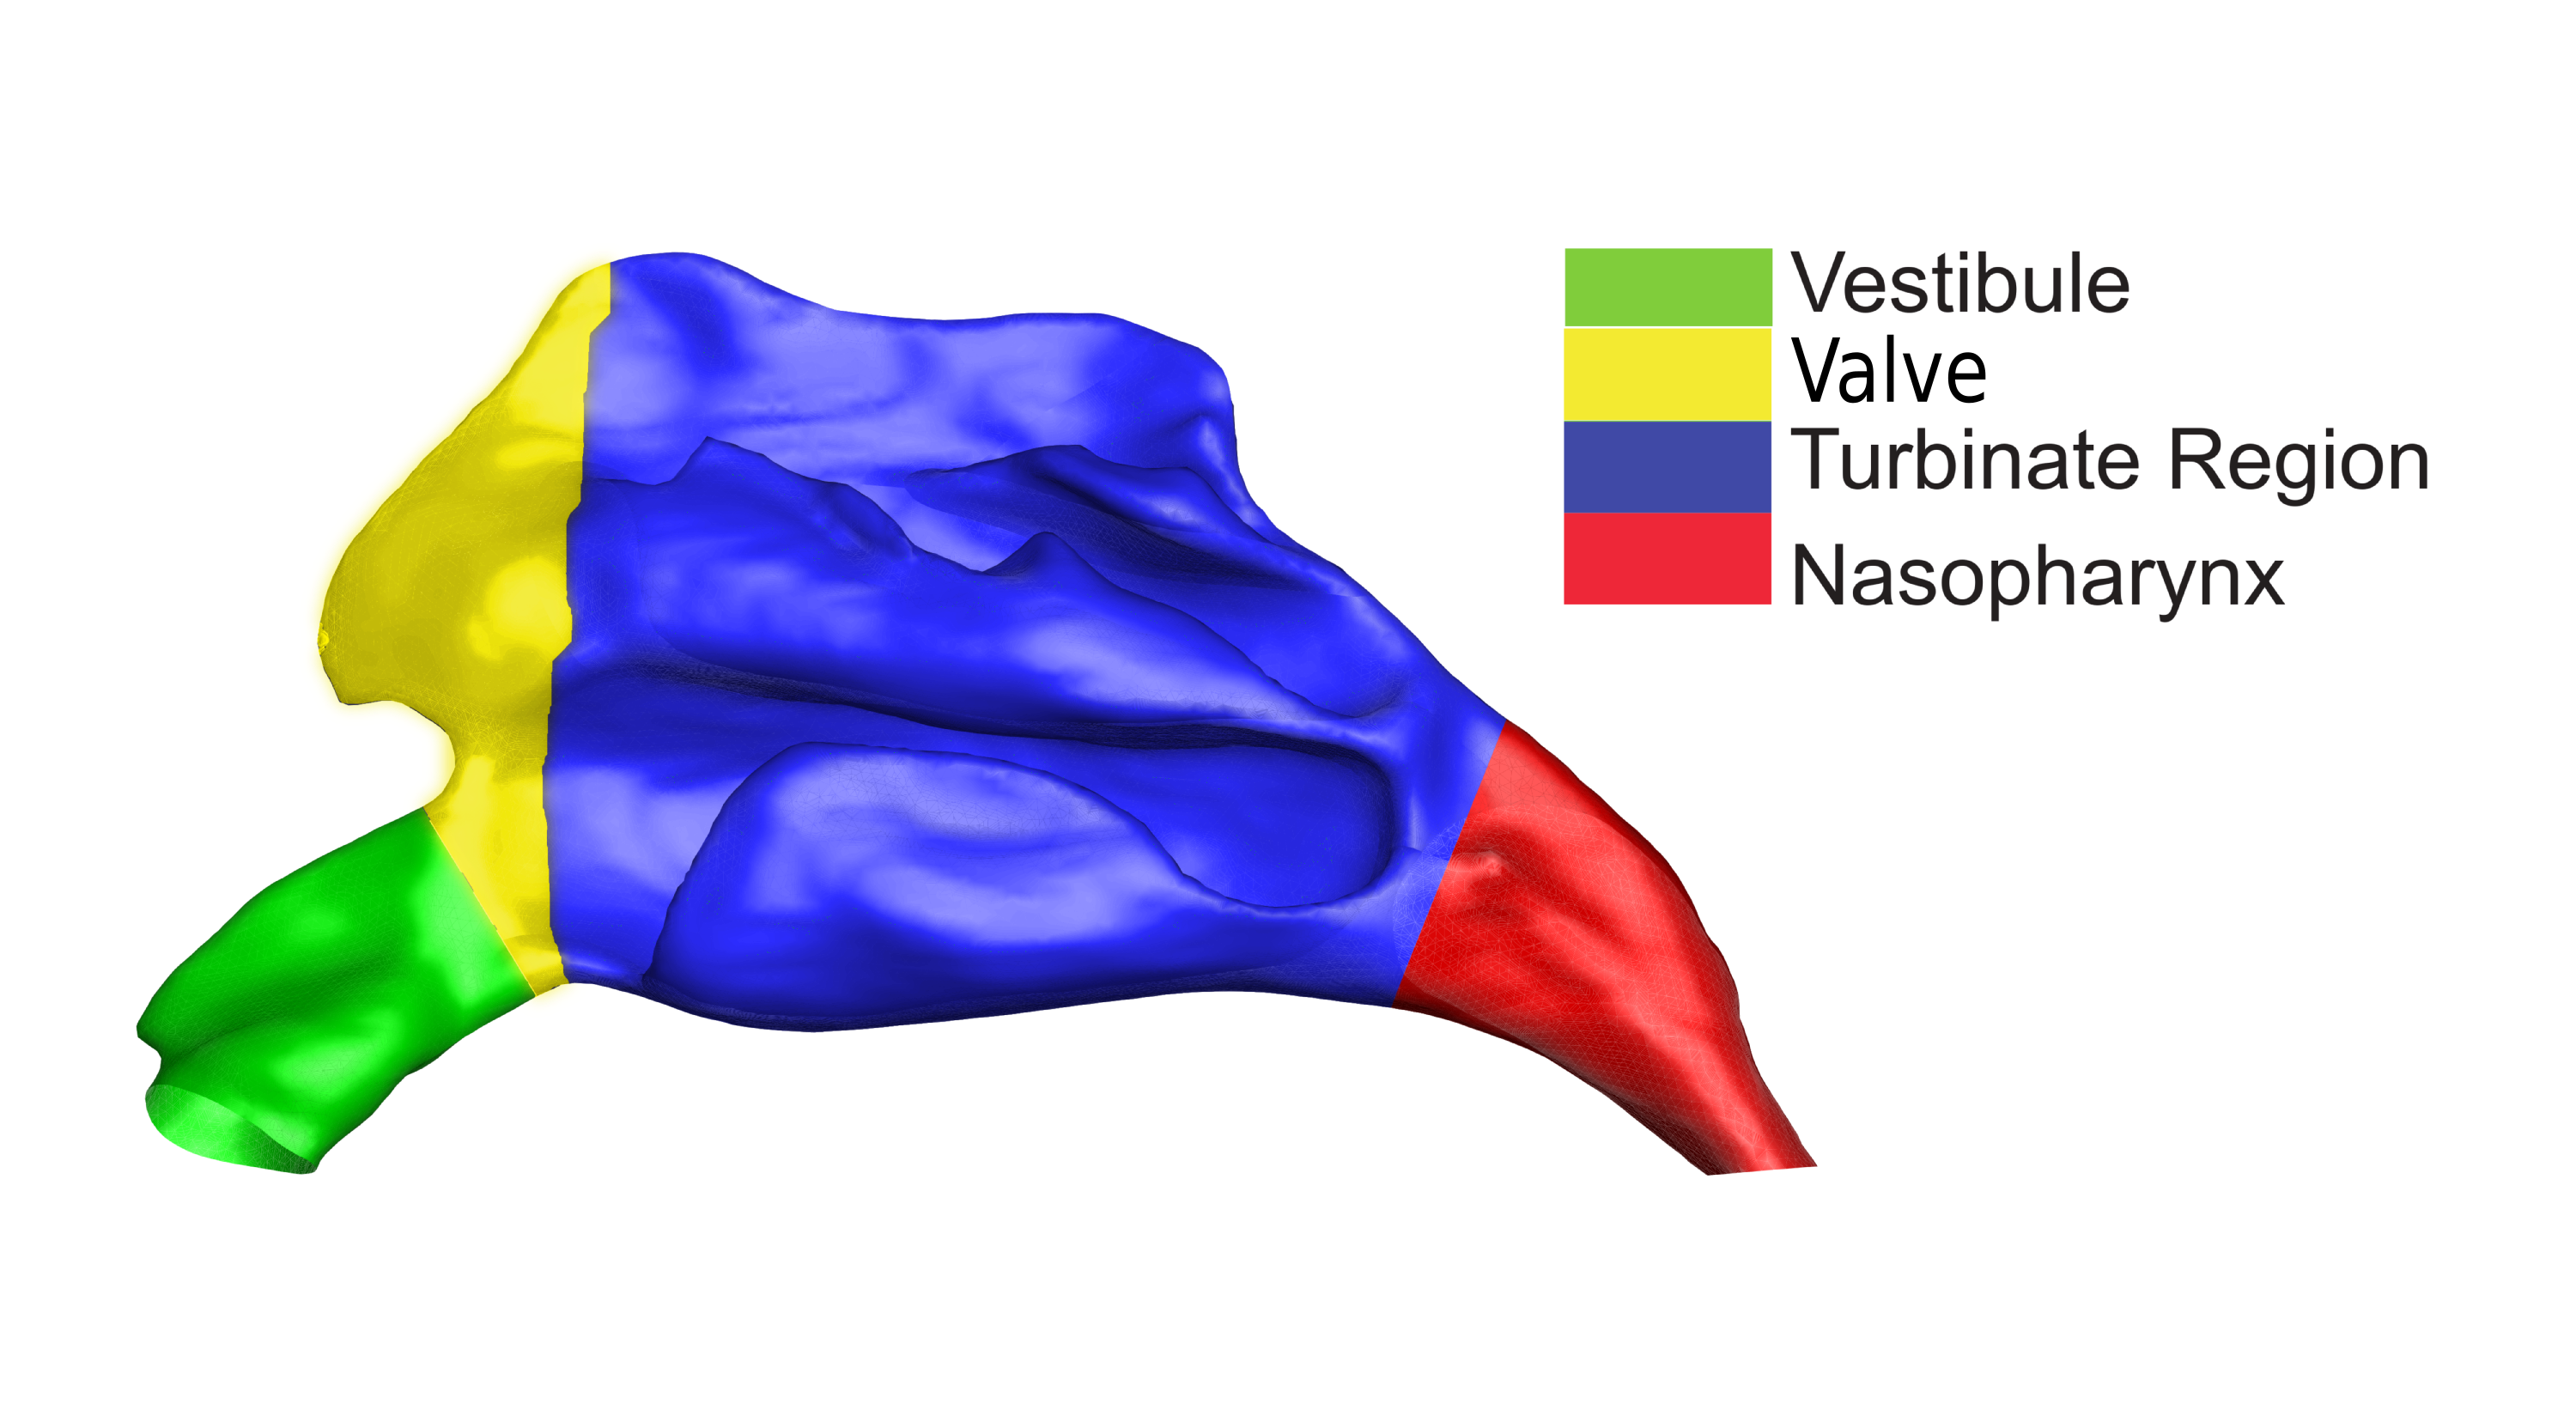
\includegraphics[width=0.7\textwidth]{regions}
\caption{Colour coded display of the anatomical regions of the nasal cavity} 
\label{fig:regions1}
\end{figure} 


The nasal cavity is the primary conduit for air coming into the respiratory system. \cite{Elad2008}. The nasal cavity consists of two 5 by 10 cm chambers running between the nostrils and the pharynx \cite{Mygind1998}. The cavities are each made up of three meatus. The meatus are connected to the nasolacrimal duct and paranasal sinuses, which are the largest of the many sinuses that surround the nasal cavity \cite{Mygind1998}. 
The nasal cavity is lined by respiratory epithelium. This epithelium controls the movement of mucous within the nasal cavity and is thus essential to its (the nasal cavity) airconditioning functionality \cite{Mygind1998}.
The two major functions of the nasal cavities are conditioning of the air for interaction with the internal airways by warming and humidification, and olfaction \cite{Doorly2008, Elad2008, Mygind1998, Berglund1982}.

\subsection{Geriatric rhinology}
Rhinology is the branch of medicine that deals with the nose and its pathologies. 
Common rhinological complaints of the elderly include dryness, runny noses, crusting and epistaxis \cite{Varga-Huettner2013}. Epidemiological studies have been carried out to examine the consistency of the manifestation of various symptoms throughout elderly patients with mixed results. 

The literature at present seems to be unanimous on the tendency of the nasal cavity's cross sectional area to increase with age. Several researchers have investigated this phenomena using acoustic rhinometry and shown good concordance in study outcomes \cite{Kalmovich2005, Edelstein1996,WhanKim2007,Lindemann2008}. Loftus et al. \cite{Loftus2016} compared the volumes of 22 nasal cavity models taken from CT scan data, and also found a clear tendency towards increased nasal cavity volume with ageing. Nasal air heating and humidification examined in vivo have been shown to be impaired in older patients; Lindemann et al. \cite{Lindemann2008} found average end-inspiratory temperature of $24^{\circ}C$ for older  patients as opposed to $27.1^{\circ}C$ for younger patients. Their findings for humidity were comparable. 

Increases in postnasal drip, nasal drainage, sneezing, coughing, olfactory dysfunction and gustatory rhinitis with age were observed in a clinical study of 131 patients \cite{Edelstein1996}. A 2009 study found that in a sample of 80 people no significant relationship could be observed between age and nasal discomfort \cite{Lindemann2010}. The same study, however, concurred with previous results on the increase of volume and cross sectional area as a function of age. Changes within the nose appear to not be limited to the increased volume; Both functional and structural variations in the respiratory epithelium have been observed with age, contributing to slower clearing of mucous \cite{HO2001}. 

Functional variations in air conditioning capabilities have been shown in vivo \cite{Lindemann2008}, with statistically significant reductions in relative humidity and heat transfer observed in elder nasal cavities. The level to which this is attributable to change in histological function as opposed to variations in the fluid mechanisms as a result of the expansion of the cavity remains to be investigated.

 \subsection{Experimental studies in rhinology}
 
To investigate air flow mechanisms in older nasal cavities, an experimental technique for the investigation must first be chosen. In this section the methods available for investigating nasal patency are presented.

The anatomy of the nasal cavity was first classified in detail by Emil Zuckerlandl in the 19th century \cite{Stammberger1989}. Anatomically, his records were more or less up to the standard of what can be assessed from modern scanning techniques \cite{Stammberger1989}, however the investigation of airflow characteristics was still severely limited by technological capacity \cite{Eccles2000}. It was not until the turn of the 19th century that experimentation in to nasal airflow began in proper \cite{Eccles2000}. 

Some of the more common in vivo techniques used include rhinomanometry, which measures of the pressure drop across the nasal cavity \cite{Hilberg1989}; and acoustic rhinometry, which allows measurement of the cross sectional area of the nasal cavity as a function of depth \cite{Hilberg1989}. 

Ultimately, however, direct detailed measurements of flow mechanics within the human nasal cavity taken in vivo are not practically viable with current technology as a result of the complexity and small scale of the nasal geometry \cite{Doorly2008c}. Thus the preferred media for the testing in modern times has tended to be either physical or computational models reconstructed from CT scan data \cite{Doorly2008c}. The physical models that have been constructed from CT scan data are able to provide detailed geometric reproductions.
These geometries can then be used to create accurate 3D models which can then be used with techniques like particle image velocimetry to conduct in detailed flow analysis throughout the nasal cavity \cite{Chung2008, Kelly2000}.
These techniques allow for data about instantaneous velocities at many points throughout a working fluid to be obtained through photographic methods. From this data the flow regime can be computed with high accuracy, allowing for in depth quantitave and qualitative analysis. Spence et al. \cite{Spence2012}, for example, showed detailed velocity contours from unsteady flow experiments using PIV.
Such experimental set ups are, however, costly to run in terms of time and resources, in particular when compared with the high level of detail that can be achieved from a well done CFD simulation \cite{Ma2009}.


\subsection{Computational studies}  
\subsubsection*{Background}
Computational fluid dynamics(CFD) is a discipline which is concerned with the computational approximation of solutions to the navier stokes equations for closed fluid systems \cite{Tu2008}. In many fields - inlcuding rhinology - CFD has facilitated economical and detailed investigations into cases in which experimental investigation would otherwise be costly or impossible \cite{Keyhani1995}.

CFD was the primary driving force behind the development of larger and faster computers until the 80's \cite{Wendt2009}. In more recent times, the continuing advancement of computational technologies has facilitated considerable growth in the scope and accuracy of CFD for predicting the behaviour of increasingly complex systems \cite{Tu2008}. 


\subsubsection*{Nasal airflow}
One of the areas of investigation that has been facilitated by these advances is that of nasal airflow. Initially, simplified nasal cavity geometry models were used to create computational meshes and solve numerically for the fluid flow characteristics under steady state state conditions \cite{Keyhani1995, Hahn1993}. Later 3D models extracted from CT scans were used to achieve more accurate results \cite{Martonen2002}. 

\subsubsection*{Boundary conditions}
Various inlet and outlet conditions have been considered, including the difference between unsteady state  (flowrate as a function of time throughout the nasal cycle) \cite{Shi2006} and steady state (constant velocity, time independent) assumption based models \cite{Wen2008}. This discrepancy has been a point of much contention, and it seems that the current position is that the correct choice depends on the application at hand \cite{Doorly2008c}. Certainly to date it seems that the vast bulk of the case studies comparing different geometries have used the steady state state assumption \cite{Xi2012, Zhu2011, Garcia2007, Doorly2008c, Keyhani1995, Subramaniam1998, Wen2008}. This assumption has been qualified on the basis of the low (below 0.2) Strouhal number for respiratory airflow \cite{Keyhani1995}, and more recently verified for certain parameters such as wall shear stress \cite{Doorly2008c}.


The flow rate for many of these steady state experiments and simulations has been determined on the basis of resting minute ventilation for healthy adults \cite{Subramaniam1998, Wen2008}. This figure tends to be recorded around 7.5 litres per minute \cite{Chaya2006, Tobin1983}. This gives an average steady flow inspiratory rate of 15 litres per minute (as the minute volume is both inhaled and exhaled during one round of respiration) \cite{Subramaniam1998}. For such flow rates the flow can be accurately treated as laminar \cite{Doorly2008c, Hahn1993}.


Another issue which has been of some debate in the literature is the relevance of the inclusion of sinuses in the modelled flow domain. It has been reasonably commonplace to include the sinuses in studies that are examining the effects of sinus surgery \cite{Xiong2008a, Lindemann2005}. Also it has been shown that, while the impact on airflow is relatively minimal, the sinuses can be subject to significant levels of particle deposition for particles in the range of 1 nanometre in diameter, and particularly for low flow rates \cite{Ge2012}. The added requirements in time and computational complexity necessitated by the inclusion of the sinuses, however, seems to warrant their exclusion from models in situations where they are not specifically relevant \cite{Doorly2008c}.


Earlier numerical models restricted their domain to the nasal cavity itself \cite{Keyhani1995, Subramaniam1998, Wen2008}. Later it was suggested that the area around the nasal vestibule is liable to influence the developement of the inlet flow distribution \cite{Doorly2008}. The facial features have also been shown to influence flow field developement \cite{Anthony2005}. More recently, facial features have been included in computational models to allow for inlet profile developement \cite{Li2012, Lee2010}.


\subsubsection*{Older nasal cavities}
Computational studies have yet to be undertaken for older nasal cavities. It is expected that the technologies available to us now for studying variations in nasal functionality could afford an unprecedented insight into their structure and function.

\subsection{Geometric variations}
The basis of any in depth investigation into the relationship between geometric variations and airflow structures is a clear analysis of the geometric variations. Various demographic factors have been suggested to influence nasal morphology, such as ethnicity; as humans evolved, nasal cavities adapted to variations in climate as to preserve optimal heat and moisture exchange in the nasal mucosa \cite{Davies1932, Thomson1923, Weiner1954, Churchill2004, Noback2011}.

Cross sectional areas have been graphed as a function of radial position to compare the geometries of different models in many studies \cite{Xi2012, Zhu2011, Lindemann2008, Garcia2007}. Surface area has also been suggested to be significant metric in predicting flow behaviour (as surface area to volume ratios are expected to impact on the flow behaviour) \cite{Xi2012, Garcia2007}. The minimum coronal cross-sectional area is a figure that has been suggested to be of particular sinificance to flow development \cite{Lindemann2008}. The ratio of area to volume (or perimeter length to cross sectional area) has been used by several researchers to predict flow characteristics \cite{Xi2012, Garcia2007}.

The lack of detailed computer based studies to date on older models means that many of these metrics and investigative techniques, are yet to be applied to older models, despite the deeper insight into their functionality that they could provide.

\subsection{Fluid dynamics}


\subsubsection{Pressure drop}

Pressure drop across the nasal cavity is widely considered to be highly corolated with sensations of nasal patency \cite{Ottaviano2016}.
The earliest papers investigating nasal patency focused primarily on the pressure drop over the nostrils, as measured with rhinomanometry \cite{Martin1981}. 
Resistance across the nasal cavity, measured as pressure drop, is still often used as a predictor of flow behaviour within the nasal cavity \cite{Edelstein1996, Lindemann2008, WhanKim2007}. 
Pressure drop has also been suggested to provide insight in to the inspirational efficiency of the cavities \cite{Lintermann2013}. 
It is often plotted as a function of flow rate in order to provide a point for validation by comparison with experimental set ups \cite{Wen2008, Inthavong2014}. 
In addition, it can be treated as a function of longitudinal position in order to gain an insight in to the relationship between the geometric variations and pressure drop \cite{Lintermann2013}. 
A selection of distributions of pressure drop as a function of flow rate, both experimentally and computationally determined, can be seen in Figure\ref{fig:pvf}. 

Pressure drop across the nasal cavity is of particular interest in older cavities, as computational analysis of the pressure drop across older cavities could assist in the understanding of the relationship between the rhinomanometry and acoustic rhinometry results for older cavities presented by previous researchers such as Lindemann et al. \cite{Lindemann2008}, who found for a transnasal pressure of 150 Pa that older patients exhibited an average flow rate of $306 cm^3/s$ as opposod to 279 for younger models.

\begin{figure}
  \centering
  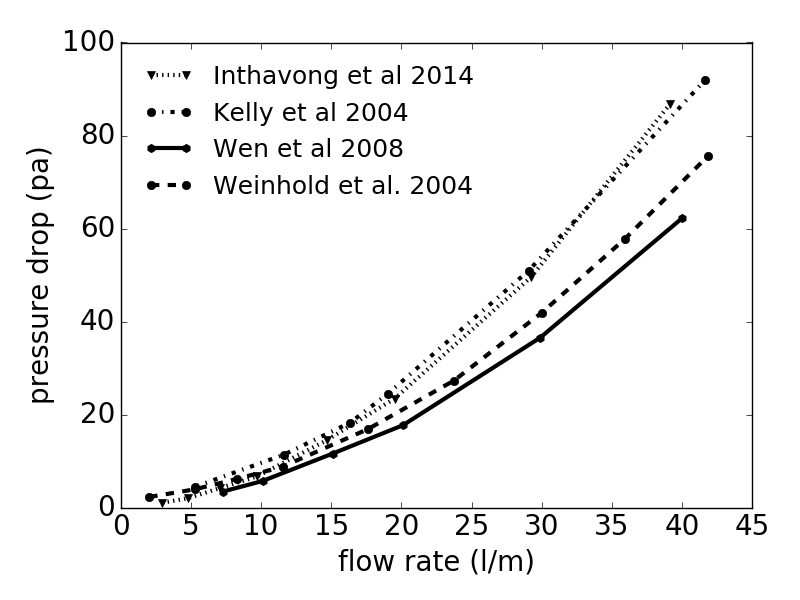
\includegraphics[width=0.8\textwidth]{pressureDrop.png}
  \caption{Pressure drop across the nasal cavity as a function of flow rate} \label{fig:pvf}
\centering
\end{figure}

 \subsubsection{Wall shear stress and velocity}

Velocity distributions in the nasal cavity play a significant role in olfaction \cite{Ishikawa2009} and Particle filtration \cite{Inthavong2006, Wang2009a} as well as general understanding of nasal function \cite{Keyhani1995, Zhu2011, Lintermann2013}. 
These can be examined by cross sectional zone by zone analysis \cite{Keyhani1995, Zhu2011}, which has been suggested to be useful for the measurement of the efficacy of olfaction \cite{Zhu2011}, or by longitudinal sections \cite{Lintermann2013,Taylor2010}. 

It has been suggested that shear stress at the wall of the nasal cavity could impact on the complex multifarious histiological mechanisms contained in the nasal epithelium \cite{Elad2006}.
Distributions are analysed longitudinally \cite{Wen2008} or around the cross sectional parameter of the relevant section of the nasal cavity \cite{Burgos2014}. 

These measurements (Wall shear and velocity) have been shown to be significant for predicting heat and mass transfer characteristics \cite{Taylor2010}, and as such their longitudinal and parametric distributions are significant for understanding the distribution of such mechanisms. 

\begin{figure}
  \centering
  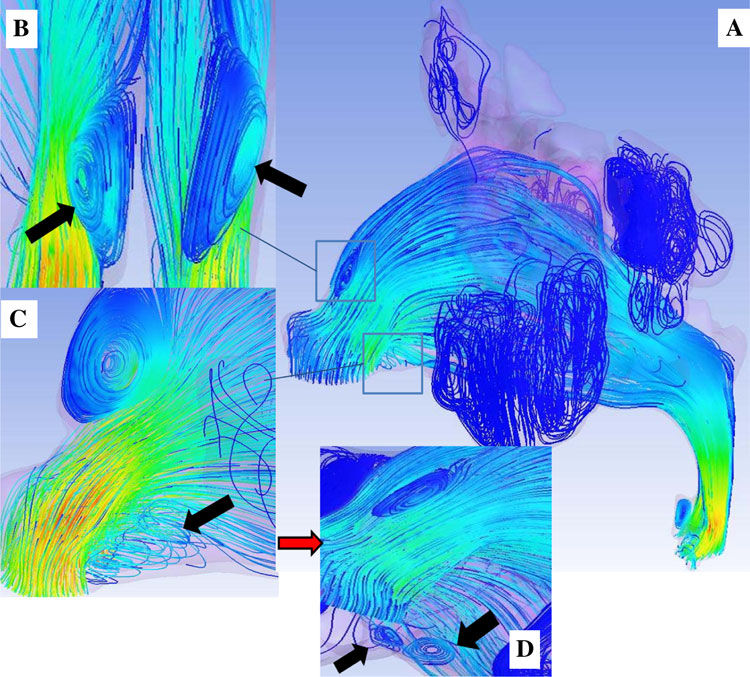
\includegraphics[width=0.6\textwidth]{chinstreams.png}
  \caption{Inspiratory airflow streamlines in the nasal cavity with sinuses coloured by velocity from Tan et al. \cite{Tan2012}} \label{fig:chinstreams}
\centering
\end{figure}

\begin{figure}
  \centering
  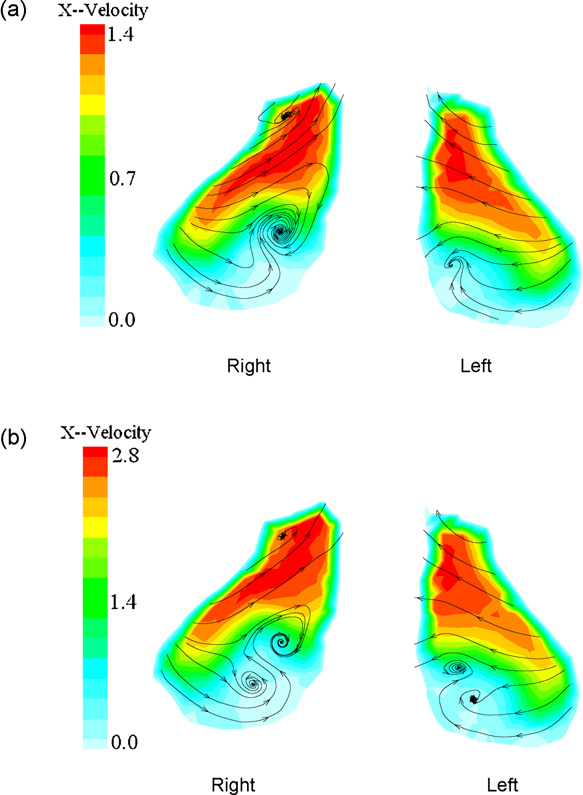
\includegraphics[width=0.4\textwidth]{wencont.png}
  \caption{Velocity contours at the nasal valve for steady state inspiratory flow rates of a) 7.5 lpm and b) 15 lpm from Wen et al. \cite{Wen2008}} \label{fig:wencont}
\centering
\end{figure}

One common visualisation method is the use of streamlines (shown in Figure \ref{fig:chinstreams}). Streamlines, often coloured by velocity \cite{Wen2008, Zhu2011, Garcia2007}, are useful for showing flow distribution as well as significant recirculation zones \cite{Lintermann2013, Xi2014}. Another commonly used method, shown in Figure \ref{fig:wencont} is coronal cross sectional contours coloured by velocity. These contours may or not include streamlines to help highlight the presence of vortices in the flow \cite{Wen2008}. Another method, presented in Lintermann et al. \cite{Lintermann2013} uses a vortex detection algorithm to trace the vortices present in the flow structure. In Lintermann et al. \cite{Lintermann2013}, these are then coloured by variables related to turbulence and vorticity in order to provide a deeper insight in to the vortex structure and behaviour.

\subsubsection{Heat and vapour transfer}

The conditioning of inhaled air - by both humidification and heating - in preparation for interaction with the sensitive tissues of the respiratory system is one of the primary functions of the nasal cavity \cite{Elad2008}.
Under standard atmospheric conditions, the air reaches an average temperature around 34\degree C and humidity of 32 $mg H_2 O/l$ by its entrance to the pharynx \cite{Keck2000}.
Interethnic variations in Nasal airconditioning effectiveness have been observed and suggested to be linked to climate related evolutionary variations \cite{Noback2011, Yokley2009}.
Reductions in airconditioning functionality in older patients have been observed experimentally \cite{Lindemann2008}.
The average temperature of the respiratory epithelium during resting nose breathing has been found to be 32.6$^{\circ} C$ \cite{Lindemann2002}.

Earlier investigations into the heat and vapour transport characteristics of the nasal cavity used a straight pipe model as a simplification of the nasal cavity geometry \cite{Ingelstedt1961}. The first experiments involving real nasal cavity geometries were carried out in the 80s, using cast models taken from cadavers \cite{Nuckols1983}.

In vivo experiments into temperature variation across the nasal cavity have been done using various temperature measuring devices; modern experiments have tended towards using thermocouples because they are small and respond quickly \cite{Elad2008}. For measuring humidity in vitro, modern researchers have tended towards the use of capacitative humidity sensors \cite{Keck2000}. Detailed profiles of temperature and humidity throughout the nasal cavity have been presented by several past researchers \cite{Keck2000}. 

CFD has been used to simulate heat and vapour transfer in the nasal cavities with good accordance with experimental results \cite{Lindemann2004}. Early simulations investigating heat and vapour transfer used a steady state assumption for inflow conditions \cite{Naftali1998}. Later, the effect of the nasal cycle on temperature distributions was investigated, showing significant variations in the nasal temperature distributions throughout the nasal cycle \cite{Elad2006}. For these simulations, the respiratory epithelium, which coats the majority of the nasal cavity, was assumed to be at 100\% relative humidity, with the exception of the interior of the nostrils, for which there was zero water flux \cite{Elad2006}.

Coronal cross section temperature contours have been used to visualise the distribution of temperature throughout the nasal cavity; this provides a clear method for visualising the distribution of temperature throughout the cross section \cite{Naftali2005}. Sagittal heat flux contours have also been used to similar effect \cite{Sullivan2013}. Heat flux, temperature, water flux and humidity have all been mapped as functions of position across the sagittal axis in the nasal cavity \cite{Garcia2007, Sullivan2013, Yu2014}. The nasal valve has been noted from these observations to be a region of particular significance to heat and vapour transfer mechanisms \cite{Sullivan2013}. 

In vivo studies looking at older nasal cavities have shown them to exhibit a reduced humidifying and heating capacity \cite{Lindemann2008}. Further investigations through computational methods into these variations could lead to more insight into the mechanisms underlying these discrepanies.

\subsection{Demographic studies}
One common application of CFD and fluid dynamics in rhinology is to investigate the effects of interdemographic variations in nasal geometry on flow features. The previously investigated demographics include ethnicity \cite{Zhu2011}; disease \cite{Garcia2007}; and  age \cite{Xi2012}. Age can be subclassified into children \cite{Xi2012} and the elderly \cite{Lindemann2008}. Both child and older nasal cavities have been investigated through in vitro \cite{Weinhold2004} and in vivo \cite{Kalmovich2005, Edelstein1996, WhanKim2007, Lindemann2008} experimental techniques. Child models have also been investigated computationally \cite{Xi2012}. The variations that have been observed in children's nasal airway functionality has been suggested to be linked to particle filtration ability \cite{Xi2012}. It seems plausible that this effect could be significant also in the case of elderly models. It is to date, however, unknown as in depth computational studies investigating flow field variations in older models are yet be undertaken.


\section{Summary}

Throughout this section, we have seen that the nasal cavity is an important organ for airconditioning as well as olfaction. We have seen that there are an assortment of ailments related to this organ which effect older patients in particular. It has been seen that there are clearly established trends between nasal cavit volume and age. We have examined the various methods available for examining the functionality of the nasal cavity. We have also looked at the use of fluid dynamics for classifying and understanding the functionality and pathology of the nasal cavity.

Although various experimental techniques have been used historically in rhinology, none of them provide the same cost effectiveness and level of detail which can be obtained through computational analysis of 3D models obtained from medical imaging. This method has been used extensively in recent years to examine various aspects of nasal cavity functionality, including interdemographic variations therein. These investigations have yielded multifarious insights into the various capacities of the organ. To date, to the best of my knowledge, the investigated demographics have not included older patients.

\section{Literature gap}

\begin{figure}
  \centering
  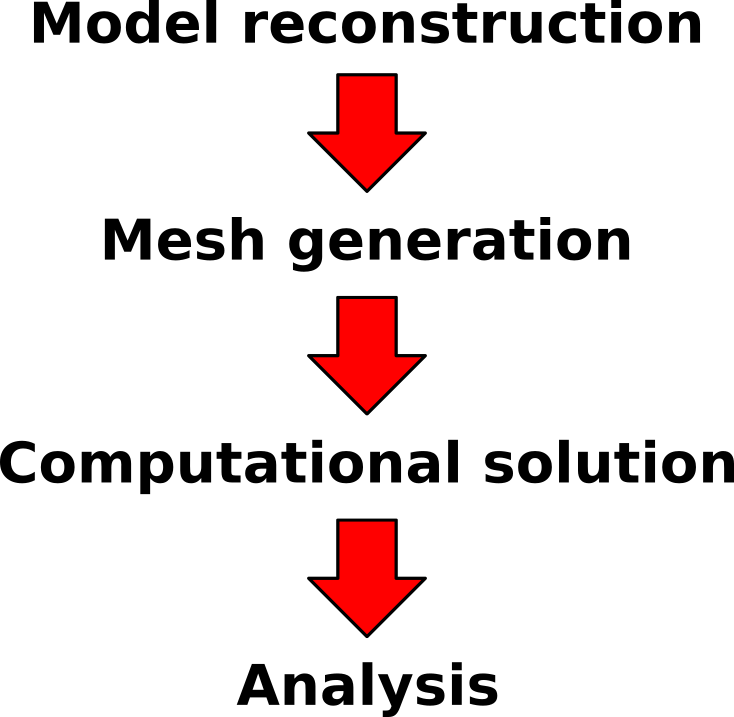
\includegraphics[width=0.6\textwidth]{probschem.png}
  \caption{Schematic overview of research}\label{fig:prbschm}
\centering
\end{figure}

On the basis of the literature review presented above, the following gaps in the current body of knowledge seem significant:

\begin{itemize}

  \item Detailed analysis of geometric discrepencies between older nasal cavities based on 3D scan models are yet to be carried out

  \item The correlations between geometric discrepencies in older nasal cavities and the airflow mechanisms induced in them through inspiration has yet to be analysed

  \item The effect of geometric discrepencies between older nasal cavities on heat and vapour transfer has yet to be assessed in detail

\end{itemize}
\section{Research questions and objectives}

In light of the information posed above, the following questions become pertinent:

\begin{itemize}

  \item How do variations in nasal cavity geometry in older Chinese Males influence the inhaled airflow mechanisms, contributing to respiratory ailments?

  \item How do the geometry variations impact on heat and vapour transfer within the cavity, contributing to respiratory ailments?

\end{itemize}

To address these issues, the following objectives are outlined:

\begin{itemize}

  \item Reconstruct a series of nasal cavity geometries from medical scans that represent a spread of geometric characteristics [such as volume and surface area] across the norm. The existing literature shows a clearly defined relationship between age and volume: these models will serve as a representative sample of the older population to be analysed computationally.

  \item Model airflow across the series of reconstructed nasal cavities using CFD with a steady state assumption; defining inlet conditions to approximate a resting rate of respiration. 

  \item Compare the simulation results between geometries. A variety of post processing methods are available to compare various aspects of fluid mechanic functionaility of nasal cavity models. The literature has shown clear discrepencies in the functionality of nasal cavities as a function of age; it is our intention through these measurements to examine in more detail the relationship between these variations and geometry.

  \item  Compare with results from the literature. 
\end{itemize}
 
\section{Research overview}

Medical image reconstruction technologies now allow researchers to reconstruct highly detailed, digital 3D representations of various anatomical structures from ct scans. When coupled with CFD simulations, this presents an unprecedented capacity for in depth analysis of physiological fluid flow mechanisms.

This study aims to use CFD analysis of CT scan data from the nasal cavities of a range of older Asian males to investigate the impact of geometric variations between older nasal cavities on the airflow structures and air-conditioning capacity of the nasal cavity. Air flow mechanisms, heat transfer rates and humidification efficacy are analysed in order to arrive at a more precise understanding of the role of nasal geometry in the presentation of respiratory ailments.

This study represents, to the best of our knowledge, the first in depth, mechanistic, computational study undertaken into the role of nasal geometry in common rhinological symptoms observed in older patients.




